For both our replication and reproduction studies we use a similar workflow, sketched in Figure~\ref{fig:methodology}. We work with git repositories, which means that we can clone the whole repository locally, and that each code snapshot corresponds to a commit in the git history of the repository. We locate repositories to analyze, clone them, and try to find out all the commits of interest. If we cannot clone a repository, or we do not find all the commits of interest in it, we discard it. Then, for each remaining repository, we get its commits of interest, and for each of these commits we investigate if it uses a building system. If so, we try to build it.

\begin{figure}[t]
\centering    
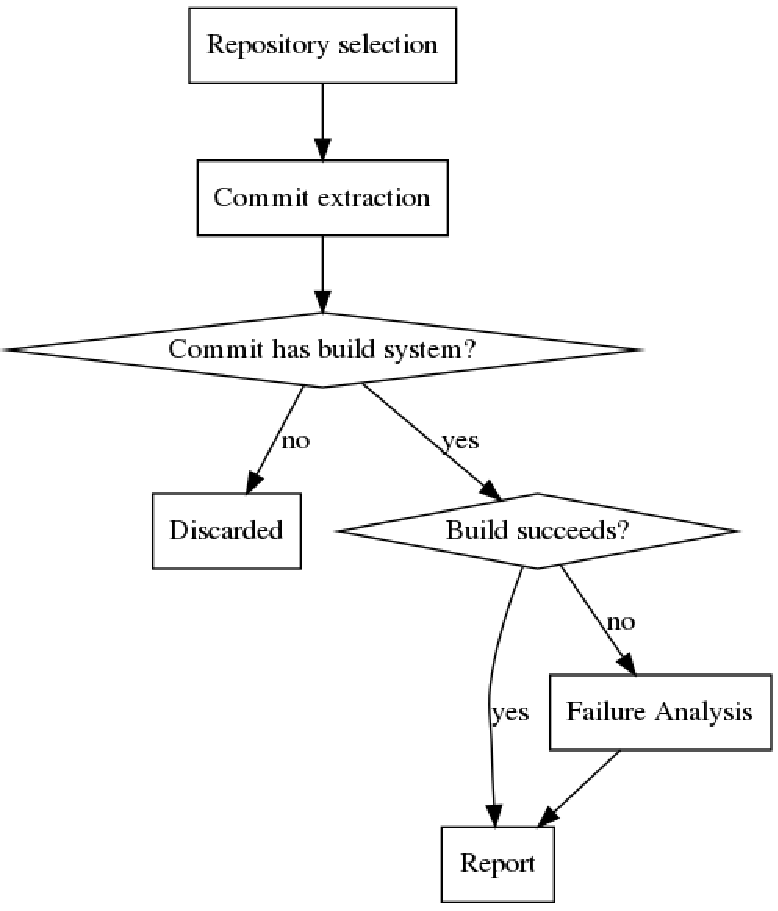
\includegraphics[height=8.5cm]{pages/01-Buildability/images/Methodology.pdf}
\caption{Basic workflow for both studies.}
\label{fig:methodology}
\end{figure}


% Reduce separation between cells in next table
\renewcommand{\tabcolsep}{3pt}

\begin{table}[h]
\caption{Studies (main quantities)}
\label{table:statistics}
\begin{center}
\begin{tabular}{lrrrr}
\toprule
\textbf{Studies:}        & \textbf{Original} & \textbf{Original} & \textbf{Replic.} & \textbf{Reprod.} \\
                         & \textbf{Pristine} & \textbf{Reduced} \\
\midrule
Repositories             & 100               & 79                & 79               & 80      \\
Commits                  & 174,505           & 139,389           & 139,389          & 300,873 \\
Commits (build conf.)    & 132,484           & 101,811           & 101,811          & 281,487 \\
Commits (build success)  & 31,696            &  22,737           & 14,664           & 98,488  \\
\bottomrule
\end{tabular}
%\caption*{
%  }
\end{center}

\begin{center}
\begin{tabular}{rrrrrrrr}
\toprule 
\textbf{Commits/project}  & \bf{min} & \bf{25\%} & \bf{50\%} & \bf{mean}  & \bf{75\%} & \bf{max}  & \bf{std} \\

\midrule
\bf{Replication}   &       25 &          234 &         726 &    1,764 &       1,898 &    14,818 & 2,694 \\
\bf{Reproduction}  &    1,132 &        1,974 &       2,980 &    3,760 &       4,847 &    10,000 & 2,404 \\


% Dejo esto aqui por si utilizamos estas cabeceras
% \bf{mean}  & 1,764.41  & 3,111.13 \\
% \bf{std}   & 2,694.93  & 1,825.44 \\
% \bf{min}   & 25       & 1,147    \\
% \bf{25\%}  & 234      & 1,791    \\
% \bf{50\%}  & 726      & 2,401    \\
% \bf{75\%}  & 1,898     & 3,693    \\
% \bf{max}   & 14,818    & 7,847    \\


\bottomrule
\end{tabular}
\end{center}

\end{table}

% Restore original separation between cells
\renewcommand{\tabcolsep}{6pt}

There are some differences between the two studies, mainly on how we find repositories, which ones are our commits of interest in them, how we find those commits, and which build systems we consider (see details below). Table~\ref{table:statistics} shows some quantification (projects and commits) for the original study, with all its projects (\textit{Original Pristine}), for the reduced version of it, with the 79 repositories in which we could find all the commits (\textit{Original Reduced}), and for our replication (considering Maven builds only) and reproduction studies. The distribution of commits per project for the replication and reproduction studies is given as well.

% % Reduce separation between cells in next table
% \renewcommand{\tabcolsep}{3pt}

% \begin{table}[h]
% \caption{Basic statistics of projects}
% \label{table:statistics}
% \begin{center}
% \begin{tabular}{rrrrrrrr}
% \toprule 
% \bf{Study}    & \bf{min} & \bf{25\%} & \bf{50\%} & \bf{mean}  & \bf{75\%} & \bf{max}  & \bf{std} \\

% \midrule
% \bf{Replication}   &       25 &          234 &         726 &    1,764.41 &       1,898 &    14,818 & 2,694.93 \\
% \bf{Reproduction}  &    1,147 &        1,791 &       2,401 &    3,111.13 &       3,693 &     7,847 & 1,825.44 \\


% % Dejo esto aqui por si utilizamos estas cabeceras
% % \bf{mean}  & 1,764.41  & 3,111.13 \\
% % \bf{std}   & 2,694.93  & 1,825.44 \\
% % \bf{min}   & 25       & 1,147    \\
% % \bf{25\%}  & 234      & 1,791    \\
% % \bf{50\%}  & 726      & 2,401    \\
% % \bf{75\%}  & 1,898     & 3,693    \\
% % \bf{max}   & 14,818    & 7,847    \\


% \bottomrule
% \end{tabular}
% \end{center}
% \end{table}

% % Restore original separation between cells
% \renewcommand{\tabcolsep}{6pt}

\subsection{Replication Study}

For the replication study we followed the methodology of the original study as much as possible. Its authors considered 100 git repositories corresponding to Java FOSS projects from the ASF, all of them using a Maven-based build infrastructure. They retrieved in September 2014 all commits in their master branches, claiming to have analyzed a total of 219,395 commits. Then, they attempted to build all of them locally using Maven. The original paper comes with an accompanying reproduction package listing in detail which commits they considered for each repository. When reviewing that list, we found that the total number of commits referenced is 174,505. This is the reason why this is the number we include in the tables for the original study (see details in Section~\ref{sec:buildability:results-repli}).

\subsubsection{Subject Recovery}

Our first step was to retrieve the git repositories to analyze. We wanted to clone all the repositories, to be able of checking out each specific commit, and analyze its compilability. We were interested in doing a replication as close as possible, so we decided to use only the repositories for which we could find all the commits of the original study. This way, we ensured that results would be comparable, and not influenced by a potentially biased sample of missing commits.

We started by using the list of git repositories from the original study to clone and check all of them. We noticed that some were not available or did not have all the commits considered in the original study. From a total of 100 repositories in the list, 6 were no longer available. Before discarding them, we tried to find them both in the ASF git repositories, and in the GitHub repositories that the foundation maintains as replicas of the original ASF-hosted ones. In addition, of those that we could clone, 19 did not have all of the commits considered in the original study (8 had none of them, 11 had only some of them). This resulted in a total of 75 repositories with the complete set of commits considered in the original study. We followed this procedure during February 2020.

To improve the number of repositories with all commits from the original study,  we turned on to Software Heritage (SH), an initiative to collect, preserve and share all public source code in a universal software archive~\cite{di2017software,di2018software}. SH tries to archive all commits, even if they are later removed from the original repositories. Therefore, it was an option for finding the missing commits. Although its API is still evolving, during March 2020 we could use it to retrieve some of the repositories with missing commits, or which we could not find\footnote{In later conversations with representatives of Software Heritage, we learned that the part of the API for retrieving full repositories had been removed because it failed in some cases, which could explain our problems in retrieving some of the repositories.}.

We found all the 25 remaining repositories in SH, but as we retrieved them using their API, 5 of them were empty or corrupt, and of the other 20, only 4 contained all the commits of the original study.

Therefore, the dataset that we used for our replication study consisted of 79 repositories out of the 100 in the original study, amounting for 139,389 commits from the total of 174,505 commits (79,9\%). Even when this is only a fraction of the commits, we consider that the sample is large enough to conduct the rest of the study, as follows.

\subsubsection{Building}

Once we cloned all git repositories, we proceeded to replicate the experiment. For that, we checked out, one by one, all source code snapshots, each one corresponding to one commit, and tried to build them. In the original study they used some Java program to run the Maven tool, via its Java API, to build the code. However, we could not find the code in their reproduction package. Because of this, but also because we wanted to produce a tooling-independent replication, we developed a Python script that uses Maven through its command-line interface. The design of the script allowed to include other build systems, to be used in the reproduction study.

\begin{figure}[t]
\centering    
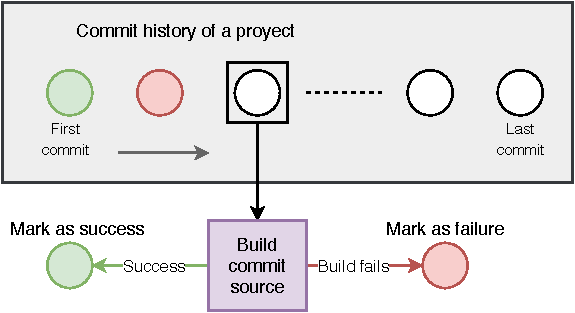
\includegraphics[width=8cm]{pages/01-Buildability/images/AnalysisProcess.pdf}
\caption{Process for checking compilability status of commits in a repository. ``Build commit source'' includes checking out the commit, checking for Maven configuration files, and if found, running Maven to try to build the code.}
\label{fig:commitHist}
\end{figure}

For each commit of interest in each repository, the script runs the following procedure (see also Figure~\ref{fig:commitHist}):
\begin{enumerate}
\item Check out the intended commit, obtaining the snapshot of the source code to be built.
\item Find the configuration for Maven (usually a \verb|pom.xml| file). If it is found, the build command for Maven is executed (\textit{mvn clean compile -X}) in a Docker container spawned for this specific analysis.
\item Collect the success code and the log produced by the execution in a log file (the verbose option of the command is used to obtain the most detailed log). If a configuration for Maven was not found, it is also noted in the log file.
\end{enumerate}

A further analysis of the log file allowed us to identify if the snapshot had configuration files for Maven, if the build was successful or not, and if not, the likely reason for the failure.

% jgb: SIZE. Remove next para if needed.
It is important to ensure the build environment is fully clean from results of previous builds, such as dependency modules or intermediate files that could influence the current one. To enforce this cleanup, besides the build command cleaning up local folders, the execution is encapsulated in a Docker container containing Maven and Java 8.

When checking for the presence of a Maven configuration file, we found an important replication issue: in all projects but three, those files were in exactly the same commits than the original study. But in those three, we found many more commits with Maven configuration (in the order of 6,000). We carefully inspected the checkout for a large sample of those commits, and our heuristics seem to work well. Unfortunately, this has some impact on the results of the replication, especially since a fraction of them are actually compilable. For having a more usable comparison with the results of the original study, we decided to analyze those commits separately (see details in Section~\ref{sec:buildability:results-repli}), so that the results on how compilability ``ages'' are not influenced because of them. That is the reason why the number of ``Commits (build conf.)'' in Table~\ref{table:statistics} is exactly the same (101,811) in both the original study (reduced) and our study (for the 79 considered repositories).

When searching for build files (pom.xml), we discovered that we were able to detect 4.72\% more commits with build files than the authors of the original study.
Detecting the presence of these build files is a relatively simple task, as they are easy to identify if they exist.
Nonetheless, to check if this inconsistency was due to an error in our scripts, we randomly selected a dozen commits where we found build files but the original study did not, and performed a manual inspection.
We found that our approach is the correct one.
So, probably the discrepancy is caused by some bug in the scripts of the original paper -- as these scripts are not publicly available, we cannot confirm this possibility.

To explore the compilability of all of the snapshots, we used two Ubuntu 18.04 machines, one of them with 16 cores and 8 GB of RAM and the other one with 8 cores and 16 GB of RAM. The software we built was capable of balancing the load between both servers to minimize execution time, building several snapshots in parallel. Once the repositories to analyze were ready, the building of all snapshots took about four weeks of wall time to run.

\subsubsection{Obtaining Results}

The results of the study are obtained from analyzing the log file. From it, we can know if a Maven configuration was found for a commit, or if the build was successful. For the analysis on the causes of build failures, we analyze the exception produced by Maven from the log for the failed builds. The exceptions that can be produced during the construction of the Maven project are well defined and limited\footnote{https://cwiki.apache.org/confluence/display/MAVEN/Errors+and+Solutions}. For the reporting, we use the classification and mapping of exceptions in the original study, which defined four categories of errors: \textit{Resolution} (related resolution of artifacts, such as downloading of dependencies), \textit{Parsing} (such as malformed build configuration), \textit{Compilation} (during the compilation phase) and \textit{Other}. Note that the first three correspond to the first three steps in the building process described in~\cite{Sulir:2016:QSJ:3001878.3001882}, presented in Section~\ref{sec:buildability:related}.

For comparing our results with the original study, we also classified every commit according to how it behaved when building it in both studies:
%\begin{itemize}
\begin{inparaenum}[\bf(1)]
  \item \textbf{stable build}, the snapshot was built in both studies;
  \item \textbf{new error}, the snapshot was built in the original study, but not in ours;
  \item \textbf{same error}, the build failed in both studies for the same reason;
  \item \textbf{different error}, the build failed in both studies but for a different reason; and,
  \item \textbf{new build}, the build failed in the original study but not in ours.
\end{inparaenum}
%\end{itemize}

We tried to reproduce the methods of the original study as much as possible, using the same classification to enable a comparison as is mandatory in a replication study.
However, we did not do it manually but automated the procedure.
We took therefore advantage of the description of the Java exceptions used in their classification by the original authors in their reproduction package\footnote{http://www.cs.wm.edu/semeru/data/breaking-changes/}.
As each exception is mapped to exactly a single category, our tool took this mapping and applied it automatically, avoiding the necessity for a manual classification.
We think this highlights one of the main reasons for replication studies: to be able to detect and fix limitations in previous works.
Our tool and data sources are publicly available in our reproduction package.


\subsection{Reproduction study}

\subsubsection{Subject selection and recovery}

For our reproduction study, we generated a new dataset of repositories to analyze. Inspired by~\cite{Sulir:2016:QSJ:3001878.3001882}, we obtained a long list of repositories via the GitHub API, meeting the following criteria:

\begin{itemize}
\item \textit{Java as the programming language}. We wanted to check Java building technologies, staying in the same domain of the original study.
\item \textit{At least 500 stars and 300 forks}. We wanted some indicator of relevance.
\item \textit{At least five years of development}. We wanted to have a long enough commit history, so that the analysis was more complete.
\item \textit{Active in January 2020} (at least one commit). We wanted projects with recent activity, to include current practices.
\item \textit{Use a build system}. We wanted to check compilability, so we checked that they were using Maven, Gradle or Ant (the three most popular build systems for Java) in the last commit.
\item \textit{Between 1,000 and 10,000 commits}. We wanted to avoid projects too small, which would have few snapshots to analyze, but also very large ones, which would consume too many resources for the analysis.
\item \textit{No Android projects}. Because of a practical limitation: building projects for Android is in general more complex, and requires specific procedures.
\end{itemize}

From the long list meeting all these conditions, we randomly selected repositories for our reproduction study and proceeded to their analysis.
For each repository, we considered all commits in the master branch as the commits of interest for the study. 
A total of 80 projects have been selected for this reproduction study.
The total number of commits was 300,873.
When comparing the resulting list with the list of projects from the original analysis, in addition to variety (since the previous analysis was focused only in ASF projects), the main difference is that we focused in non-small projects with certain relevance.

\subsubsection{Building}

The process we followed to explore the buildability of snapshots for the repositories in our list was very similar to the one described above for the replication study. The differences were as follows:

\begin{itemize}
\item After checking out a commit, three systems are considered when searching for build configuration (see ``Build File'' in Table~\ref{table:buildSystems}). In the replication study only Maven was considered.
\item When building the snapshot with more than one build system, we tried the build systems in order: first Maven or Gradle, and if it failed, then Ant. We did not find snapshots with both Maven and Gradle. Having Ant and one of Maven or Gradle is usually due to the project transitioning from the former to the latter, thus still having the old Ant configuration and a new configuration for Maven or Gradle. Our order for testing systems considers that if the Maven or Gradle configuration worked, the project had likely already transitioned to them -- if it did not, the project was still with Ant.
\item For each build configuration, we executed the build command defined by the build configuration (see ``Command'' in Table~\ref{table:buildSystems}).
\end{itemize}

\begin{table}[h]
  \caption{Build systems considered in the reproduction study}
  \label{table:buildSystems}
  \centering
  \begin{tabular}{lll}
    \toprule
    \bf{Build } & \bf{Command} & \bf{Build}\\
    \bf{System} &              & \bf{File }\\ 
    \midrule
    Maven & mvn clean compile -X & pom.xml\\
    Gradle & ./gradlew build -x test & build.gradle \\
    Ant & ant compile  & build.xml \\
    \midrule
  \end{tabular}
\end{table}
 
For this reproduction study, the Docker container we used included Java 8, Ant and Maven, while Gradle was run standalone (since it works self-contained). 
%Once the repositories to analyze were ready, 
The building of all snapshots took about two weeks of wall time, in the same environment we used for the replication study.


\subsubsection{Obtaining results}

As we did for the replication study, the results of the reproduction study are obtained by analyzing the logs of the attempts to build each considered commit from our list of repositories. The analysis is the same that we described already, with the difference that in the reproduction study we considered not only if the snapshot could be built or not, but also which build system was used. We also had to extend the mapping of exceptions in error logs to one of the four categories of errors in the original study (\textit{Dependency}, \textit{Parsing}, \textit{Compiling} or \textit{Other}). 
The new error mapping will be shown in the following sections,as well as being available in the reproduction package.
